%%
%%  Examples of a widetext environment for setting wide equations in the asmeconf class.
%%  Copyright (c) 2021 John H. Lienhard.  Use under the MIT license: https://ctan.org/license/mit 
%%
%%  USAGE: 	* \begin{widetext} ...wide material here... \end{widetext}
%%	OPTIONAL ARGUMENTS: 
%%			* \begin{widetext[N] .. changes upper/lower separation of wide material from default 5pt to Npt
%%			* \begin{widetext}[][tbn]: t = top line only; b = bottom line only; n = no lines.  BOTH arguments are REQUIRED, even if first is left empty.
%%
%%  asmewide,sty supports one option, [raggedend], which suppresses final page column balancing: \usepackage[raggedend]{asmewide}
%%
%%	The widetext environment can only appear once per page. It clashes with floats and footnotes, as discussed herein.
%%
%%  NB: the strip environment from cuted is incompatible with the [lineno] option to asmeconf!

\documentclass[nofoot,colorlinks,balance,pdf-acolorlinks,balance,pdf-a]{asmeconf}

\def\ACwidetextversion{1.1}
\def\ACwidetextdate{September 14, 2022} 

\usepackage{lipsum}% Latin filler text
\usepackage{asmewide}

\begin{filecontents}{asme-wide-equations.bib}
@online{lienhard2021,
  author = {Lienhard, John H., V},
  title = {{\texttt{asmeconf}}: A template for {ASME} conference papers},
  organization = {Comprehensive \TeX\ Archive Network},
  version = {{\versionno}},
  year = {2021},
  url = {https://ctan.org/pkg/asmeconf},
  urldate = {{\today}},
}      
@online{tolucsis1,
  author = {Sigitas Tolu\v{s}is},
  year = {2021},
  title = {The \texttt{cuted} package},
  version = {2.0},
  organization = {Comprehensive \TeX\ Archive Network},
  url = {https://ctan.org/pkg/cuted},
  urldate = {Dec. 30, 2021},
}
@online{tolucsis2,
  author = {Sigitas Tolu\v{s}is},
  year = {2021},
  title = {The \texttt{sttools} collection},
  version = {3.0},
  organization = {Comprehensive \TeX\ Archive Network},
  url = {https://ctan.org/pkg/sttools},
  urldate = {Dec. 30, 2021},
}
@book{stakgold,
author = {Ivar Stakgold},
title = {Boundary Value Problems of Mathematical Physics},
year = {1967},
publisher = {Macmillan},
address = {New York},
}
\end{filecontents}

\hypersetup{%
	pdfauthor={John H. Lienhard},                       		     
	pdftitle={Wide Equations in asmeconf.cls},                 
	pdfkeywords={ASME conference paper, LaTeX template, wide equations, widetext},
	pdfsubject = {Examples of setting wide equations in the asmeconf LaTeX template},
	pdfurl={https://ctan.org/pkg/asmeconf},
	pdflicenseurl={https://ctan.org/pkg/asmeconf},
}

%%%%%%%%%%%%%%%%%%%%%%%%%%%%%%%%%%%%%%%%%%%%%%%%%%%%%%%%%%%%%%%%%%%%%%%%%%%%%%%%%%%%%%%%%%%%%%%%%%%%%%%
\begin{document}

\ConfName{Proceedings of the \texttt{asmeconf}\linebreak International Examples Congress and Exposition}
\ConfAcronym{AIECE22}
\ConfDate{January 10, 2022}
\ConfCity{Cambridge, MA}
\PaperNo{AIECE2022-0003}

\SetAuthors{John H.\ Lienhard V\affil{}\CorrespondingAuthor{lienhard@mit.edu}}
\SetAffiliation{}{Fellow of ASME \\
Rohsenow Kendall Heat Transfer Laboratory, \\
Department of Mechanical Engineering,\\
Massachusetts Institute of Technology, \\
Cambridge, MA 02139 USA 
}

\title{Wide Equations in asmeconf.cls}
\maketitle

\versionfootnote{Examples of \texttt{widetext} in \texttt{asmeconf}. Version \ACwidetextversion, \ACwidetextdate}

\keywords{ASME conference paper, \LaTeX\ template, wide equations, asmeconf}
    
\begin{abstract}
This paper gives several examples of typesetting very wide equations with {\upshape\LaTeX} in the {\upshape\texttt{asmeconf}} class~{\upshape\cite{lienhard2021}} using {\upshape\texttt{asmewide.sty}}.
The style defines a the {\upshape\texttt{widetext}} environment, built on the 2021 release of {\upshape\texttt{cuted.sty}~\cite{tolucsis1}} from the
{\upshape\texttt{sttools}} bundle~{\upshape\cite{tolucsis2}}, which is available from CTAN, \hrefurl{http://ctan.org}{ctan.org}.  
Significant hand-fitting around pagebreaks, floats, and footnotes is required to obtain good results. Users can change the source file to explore the behavior and limitations of the {\upshape\texttt{widetext}} environment. \textcolor{red}{Only the text in \textbf{red} in this document meant 
to be read---the rest is simply filler to aid in layout.}
\end{abstract}


\section{Introduction}
\lipsum[1-2]
\section{Section}
\lipsum[3]

%%%%%%%%%%%%%%%%%  begin two column figure  %%%%%%%%%%%%%%%%%%%%%%%%%%%
\begin{figure*}[t]
\begin{subfigure}[c]{0.495\textwidth}
\centering{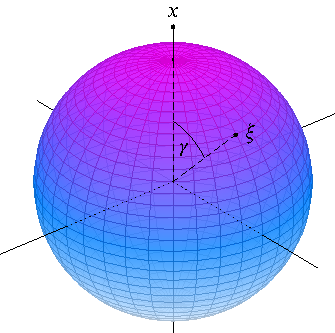
\includegraphics{zonal-harmonic2.pdf}}%
\subcaption{\label{fig:zonal}}
\end{subfigure}
%%%%%%%% don't leave a break here
\begin{subfigure}[c]{0.495\textwidth}
\centering{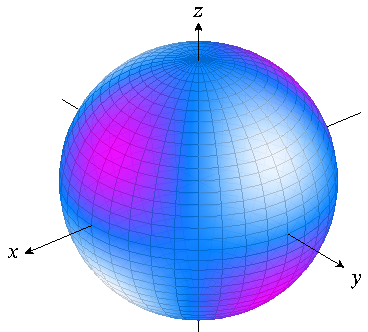
\includegraphics{tesseral-harmonic.pdf}}%
\subcaption{\label{fig:tesseral}}%
\end{subfigure}%
\caption{A figure with two subfigures: (a) Zonal harmonic $n=1, m=0$, (b) Tesseral harmonic $n=2, m=3$. See Appendix~\ref{sec:sph-har}.}\label{fig:1}
\end{figure*}
%%%%%%%%%%%%%%%%%%%  end two column figure  %%%%%%%%%%%%%%%%%%%%%%%%%%%%%

\lipsum[4]
\subsection{Subsection}
\lipsum[5-6]

%%%%%%%%%%%%%%%%%%%%  Example WT1  %%%%%%%%%%%%%%%%%%%%%%%%%%%%%%%%%%%%%%
\section{Single Wide Equation on the Page}

\textcolor{red}{Equation~\eqref{eqn:WT1} is an equation with a matrix that is too large to fit into one column. A multiline math environment will not help because the equation cannot be broken into parts that each fit into a column. The \texttt{widetext} environment solves the problem.}  

\textcolor{red}{A two-column wide figure, Fig.~\ref{fig:1}, has floated from a previous page to the top of this page, but does not interfere with the \texttt{widetext} material (a one column float would interfere).}

\begin{widetext}
\begin{equation}\label{eqn:WT1}
\mathbf{WT1:}\quad
\mathfrak{W}(\bm{\Phi})= \begin{Vmatrix}
\dfrac\varphi{(\varphi_1,\varepsilon_1)}			& 0 												& \hdotsfor{4} 	& 0 			&	\\[\jot]
\dfrac{\varphi k_{21}}{(\varphi_2,\varepsilon_1)}	& \dfrac\varphi{(\varphi_2,\varepsilon_2)}			& 0 			& \hdotsfor{3} 	& 0 \\[\jot]
\dfrac{\varphi k_{31}}{(\varphi_3,\varepsilon_1)}	&\dfrac{\varphi k_{32}}{(\varphi_3,\varepsilon_2)}	& \dfrac\varphi{(\varphi_3,\varepsilon_3)}& 0 & \hdotsfor{2} & 0 \\[\jot]
\vdots 	&  &  & \smash{\rotatebox{15}{$\ddots$}} &  & & \vdots \\[\jot]
\dfrac{\varphi k_{n-2\, 1}}{(\varphi_{n-2},\varepsilon_1)}	&
\dfrac{\varphi k_{n-2\, 2}}{(\varphi_{n-2},\varepsilon_2)}	&\hdotsfor{1} & \dfrac{\varphi k_{n-2\,n-3}}{(\varphi_{n-2},\varepsilon_{n-3})} & \dfrac\varphi{(\varphi_{n-2},\varepsilon_{n-2})}& 0& 0 \\[\jot]
\dfrac{\varphi k_{n-1\, 1}}{(\varphi_{n-1},\varepsilon_1)}	& \dfrac{\varphi k_{n-1\, 2}}{(\varphi_{n-1},\varepsilon_2)} &\hdotsfor{2} & 
\dfrac{\varphi k_{n-1\,n-2}}{(\varphi_{n-1},\varepsilon_{n-2})}& \dfrac{\varphi}{(\varphi_{n-1},\varepsilon_{n-1})} & 0 \\[\jot]
\dfrac{\varphi k_{n1}}{(\varphi_n,\varepsilon_1)}	& \dfrac{\varphi k_{n2}}{(\varphi_n,\varepsilon_2)}	& \hdotsfor{3}	&
\dfrac{\varphi k_{n\,n-1}}{(\varphi_n,\varepsilon_{n-1})} & \dfrac{\varphi}{(\varphi_n,\varepsilon_n)}
\end{Vmatrix}
\end{equation}
\end{widetext}

\lipsum[7-8]


%%%%%%%%%%%%%%%%%%%%  Examples WT2 & WT3  %%%%%%%%%%%%%%%%%%%%%%%%%%%%%%%%%%%%
\section{Two Wide Equations on the Page}

\lipsum[9-10]

\begin{widetext} 
\begin{equation}\mathbf{WT2:}
\int_a^b\biggl\{\int_a^b[f(x)^2g(y)^2+f(y)^2g(x)^2]
 -2f(x)g(x)f(y)g(y)\,dx\biggr\}\,dy
 \ne \frac{1}{\sqrt{\int_a^b\biggl\{g(y)^2\int_a^bf^2+f(y)^2
  \int_a^b g^2-2f(y)g(y)\int_a^b fg\biggr\}\,dy}}
\end{equation}

\textcolor{red}{In this case, we have a pair of wide equations on the same page.  The \texttt{widetext} environment cannot be used twice on the same page! To resolve the conflict, we remain in single column mode between the two equations.}

\textcolor{red}{This page also includes a single column float, Table~\ref{tab:2}. This float must come after the \texttt{widetext} environment. We use the \texttt{\textbackslash begin\{table\}[b]} option to force the table to the bottom of the column. The two column table, Table~\ref{tab:4}, floats to the top of the next page and creates no problems.}

\begin{equation}\mathbf{WT3:}
\int_a^b\biggl\{\int_a^b[f(x)^2g(y)^2+f(y)^2g(x)^2]
 -2f(x)g(x)f(y)g(y)\,dx\biggr\}\,dy
 \ne \frac{1}{\sqrt{\int_a^b\biggl\{g(y)^2\int_a^bf^2+f(y)^2
  \int_a^b g^2-2f(y)g(y)\int_a^b fg\biggr\}\,dy}}
\end{equation}
\end{widetext}


%%%%%%%%%%%%%%% begin single column table %%%%%%%%%%%%%%%%%%%%%%
\begin{table}[b]
\caption{Table with more complicated columns}\label{tab:2}%
\centering{%
\begin{tabular}{!{\hspace*{0.5cm}} >{\raggedright\hangindent=1em} p{3cm} d{3} @{\hspace*{1cm}} d{3} !{\hspace*{0.5cm}}}
\hline\hline
\rule{0pt}{10pt} Experiment & \multicolumn{1}{c@{\hspace*{1cm}}}{$u$ [m/s]} & \multicolumn{1}{c!{\hspace*{0.5cm}}}{$T$ [\textdegree C]} \\[1pt]
\hline
The first experiment we ran this morning   & 124.3     &   68.3   \rule{0pt}{10pt} \\
The second experiment we ran this morning  &  82.50    &  103.46  \\
Our competitor's data                      &  72.321   &  141.384 \\[1pt]
\hline\hline
\end{tabular}
}
\end{table}
%%%%%%%%%%%%%%%% end table  %%%%%%%%%%%%%%%%%%%%%%%%%%%%%%%%%%%% 

%%%%%%%%%%%%%%% begin two column table %%%%%%%%%%%%%%%%%%%%%%%%% 
\begin{table*}[t]
\caption{A table spanning two columns}\label{tab:4}%
\centering{%
\begin{tabular*}{0.8\textwidth}{@{\hspace*{1.5em}}@{\extracolsep{\fill}}ccc!{\hspace*{3.em}}ccc@{\hspace*{1.5em}}}
\hline\hline
\multicolumn{1}{@{\hspace*{1.5em}}c}{$x$\rule{0pt}{11pt}} &
\multicolumn{1}{c}{$\textrm{erf}(x)$} &
\multicolumn{1}{c!{\hspace*{3.em}}}{$\textrm{erfc}(x)$} &
\multicolumn{1}{c}{$x$} &
\multicolumn{1}{c}{$\textrm{erf}(x)$} &
\multicolumn{1}{c@{\hspace*{1.5em}}}{$\textrm{erfc}(x)$} \\ \hline
0.00 & 0.00000 & 1.00000 & 1.10 & 0.88021 & 0.11980\rule{0pt}{11pt} \\
0.05 & 0.05637 & 0.94363 & 1.20 & 0.91031 & 0.08969 \\
0.10 & 0.11246 & 0.88754 & 1.30 & 0.93401 & 0.06599 \\
0.15 & 0.16800 & 0.83200 & 1.40 & 0.95229 & 0.04771 \\
0.20 & 0.22270 & 0.77730 & 1.50 & 0.96611 & 0.03389 \\
0.30 & 0.32863 & 0.67137 & 1.60 & 0.97635 & 0.02365 \\
0.40 & 0.42839 & 0.57161 & 1.70 & 0.98379 & 0.01621 \\
0.50 & 0.52050 & 0.47950 & 1.80 & 0.98909 & 0.01091 \\
0.60 & 0.60386 & 0.39614 & 1.82\makebox[0pt][l]{14} & 0.99000 & 0.01000 \\
0.70 & 0.67780 & 0.32220 & 1.90 & 0.99279 & 0.00721 \\
0.80 & 0.74210 & 0.25790 & 2.00 & 0.99532 & 0.00468 \\
0.90 & 0.79691 & 0.20309 & 2.50 & 0.99959 & 0.00041 \\
1.00 & 0.84270 & 0.15730 & 3.00 & 0.99998 & 0.00002 \\[2pt]
\hline\hline
\end{tabular*}
}
\end{table*}
%%%%%%%%%%%%%%%% end table %%%%%%%%%%%%%%%%%%% 

\lipsum[17-23]

\lipsum[24]

%%%%%%%%%%%%%%%%%%%%  Examples WT4 & WT5  %%%%%%%%%%%%%%%%%%%%%%%%%%%%%%%%%%%%%%%%%%
\section{Wide Equation Pair Split Across Page Break and Followed by Wide Equation}

\textcolor{red}{Note that the upper rule is cleared after the first use in a \texttt{widetext} environment. This means that it will not show up at the top of the next page.}

\textcolor{red}{The \texttt{\textbackslash newpage} command may optionally be used between the equations to force the second one onto the following page, e.g., try removing the source code line \texttt{\textbackslash lipsum[24]} with and without \texttt{\textbackslash newpage}.}

\begin{widetext}
\begin{equation}\mathbf{WT4:}
\int_a^b\biggl\{\int_a^b[f(x)^2g(y)^2+f(y)^2g(x)^2] -2f(x)g(x)f(y)g(y)\,dx\biggr\}\,dy
 \ne \frac{1}{\sqrt{\int_a^b\biggl\{g(y)^2\int_a^bf^2+f(y)^2 \int_a^b g^2-2f(y)g(y)\int_a^b fg\biggr\}\,dy}}
\end{equation}%\newpage
\begin{equation}\mathbf{WT5:}
\int_a^b\biggl\{\int_a^b[f(x)^2g(y)^2+f(y)^2g(x)^2]
 -2f(x)g(x)f(y)g(y)\,dx\biggr\}\,dy
 \ne \frac{1}{\sqrt{\int_a^b\biggl\{g(y)^2\int_a^bf^2+f(y)^2
  \int_a^b g^2-2f(y)g(y)\int_a^b fg\biggr\}\,dy}}
\end{equation}

\textcolor{red}{In this case, we again have a pair of wide equations on the same page, so we stay in single column mode
until both are done\footnotemark. The single column table, Table~\ref{tab:3}, is forced to the bottom of the page using the \texttt{[b]} option.}

\lipsum[32-33]

\begin{equation}\mathbf{WT6:}
\int_a^b\biggl\{\int_a^b[f(x)^2g(y)^2+f(y)^2g(x)^2]
 -2f(x)g(x)f(y)g(y)\,dx\biggr\}\,dy
 \ne \frac{1}{\sqrt{\int_a^b\biggl\{g^2\int_a^bf^2+f^2
  \int_a^b g^2-2fg\int_a^b fg\biggr\}\,dy}}
\end{equation}
\end{widetext}
\footnotetext{\textcolor{red}{The code from \texttt{cuted.sty} doesn't play well with footnotes, so we issue a \texttt{\textbackslash footnotemark} command inside the wide material and a separate \texttt{\textbackslash footnotetext\{..\}} command outside the wide environment.}}%
\lipsum[34-37]

%%%%%%%%%%%%%%%%%%%  begin linewidth table  %%%%%%%%%%%%%%%%%%%%%%%%%%%%%%
\begin{table}[b]
\newcolumntype{C}{>{$}c<{$}} % math-mode version of "c" column type, from array package
\caption{Table at full column width with columns in math mode}\label{tab:3}
\centering{%
\begin{tabular*}{\linewidth}{@{\extracolsep{\fill}}CCCC@{\extracolsep{\fill}}}
\hline\hline
X_{z} & X_{c} & X_{c,m} & X_{c,2}\rule{0pt}{11pt}\\
 3.92069  & 5.70943 & 6.32429 & 7.08757\\[2pt]
\varepsilon (T_1)  & \varepsilon^i (T_1) & \varepsilon^i (T_m) & \alpha (T_1, T_2)\\
0.7258 & 0.6237 & 0.6807 & 0.7964 \\[2pt]
q_\textrm{gray}  & q_\textrm{int, $T_1$} & q_\textrm{int, $T_m$} & q_\textrm{exact}\\
400.2 & 462.1 & 371.0 & 371.8 \\[1pt]
\hline\hline
\end{tabular*}
}
\end{table}
%%%%%%%%%%%%%%%%%%%%  end linewidth table %%%%%%%%%%%%%%%%%%%%%%%

\lipsum[40-48]

\textcolor{red}{For eqn.~\eqref{eqn:WT7}, we drop the bottom line, keeping the top line and increasing the vertical space a bit: \texttt{\textbackslash begin\{widetext\}[8][t]}.}

\begin{widetext}[8][t]
\begin{equation}\label{eqn:WT7}
\mathbf{WT7:}\quad
\cfrac{1}{1+ \cfrac{1}{abcxyz+(ax^2-by^3+cz^4)(\alpha\chi^2-\beta\upsilon^3+\kappa\zeta^4)(ax^4-by^3+cz^2)(a^2x^2-by^3+c^2z^2)}}
\end{equation}
\end{widetext}

\lipsum[50-60]

\textcolor{red}{In the following example, we leave out the top line: \texttt{\textbackslash begin\{widetext\}[][b]}.}

\vskip 80pt% <== an extra skip to push this widetext over the edge

\begin{widetext}[][b]
\begin{equation}\label{eqn:WT8}
\mathbf{WT8:}\quad
\mathfrak{W}(\bm{\Phi})= \begin{Vmatrix}
\dfrac\varphi{(\varphi_1,\varepsilon_1)}			& 0 												& \hdotsfor{4} 	& 0 			&	\\[\jot]
\dfrac{\varphi k_{21}}{(\varphi_2,\varepsilon_1)}	& \dfrac\varphi{(\varphi_2,\varepsilon_2)}			& 0 			& \hdotsfor{3} 	& 0 \\[\jot]
\dfrac{\varphi k_{31}}{(\varphi_3,\varepsilon_1)}	&\dfrac{\varphi k_{32}}{(\varphi_3,\varepsilon_2)}	& \dfrac\varphi{(\varphi_3,\varepsilon_3)}& 0 & \hdotsfor{2} & 0 \\[\jot]
\vdots 	&  &  & \smash{\rotatebox{15}{$\ddots$}} &  & & \vdots \\[\jot]
\dfrac{\varphi k_{n-2\, 1}}{(\varphi_{n-2},\varepsilon_1)}	&
\dfrac{\varphi k_{n-2\, 2}}{(\varphi_{n-2},\varepsilon_2)}	&\hdotsfor{1} & \dfrac{\varphi k_{n-2\,n-3}}{(\varphi_{n-2},\varepsilon_{n-3})} & \dfrac\varphi{(\varphi_{n-2},\varepsilon_{n-2})}& 0& 0 \\[\jot]
\dfrac{\varphi k_{n-1\, 1}}{(\varphi_{n-1},\varepsilon_1)}	& \dfrac{\varphi k_{n-1\, 2}}{(\varphi_{n-1},\varepsilon_2)} &\hdotsfor{2} & 
\dfrac{\varphi k_{n-1\,n-2}}{(\varphi_{n-1},\varepsilon_{n-2})}& \dfrac{\varphi}{(\varphi_{n-1},\varepsilon_{n-1})} & 0 \\[\jot]
\dfrac{\varphi k_{n1}}{(\varphi_n,\varepsilon_1)}	& \dfrac{\varphi k_{n2}}{(\varphi_n,\varepsilon_2)}	& \hdotsfor{3}	&
\dfrac{\varphi k_{n\,n-1}}{(\varphi_n,\varepsilon_{n-1})} & \dfrac{\varphi}{(\varphi_n,\varepsilon_n)}
\end{Vmatrix}
\end{equation}
\end{widetext}

\lipsum[55-56]

%%%%%%%%%%%%%%%%%%%%%%%%%%%%%%%%%%%%%%%%%%%%%%%%
\appendix  
\section{Spherical harmonics}\label{sec:sph-har}

Without getting into the details, a regular function $f(\theta,\phi)$ on the surface of the unit sphere may be written
\begin{equation}
f(\theta,\phi) = \sum_{n=0}^\infty \sum_{m=-n}^n f_{m,n} Y_n^m(\theta,\phi)
\end{equation}
for $Y_n^m(\theta,\phi) = e^{i m\phi}P^{|m|}_n(\cos\theta)$, for $|m|<n$. The case $n=3$, $m=2$ (a \textit{tesseral harmonic}) is shown in Fig.~\ref{fig:tesseral}.

These functions are orthogonal, with the normalization constant~\cite[App.~A]{stakgold}:
\begin{equation}
N_{m,n}=\int_0^{2\pi}\!\!d\phi\int_0^{\pi}\!\!d\theta \sin\theta\, \big|Y^m_n(\theta,\phi)\big|^2 = \frac{4\pi (n+|m|)!}{(2n+1)(n-|m|)!}
\end{equation} 

If $f$ is independent of the azimuthal angle $\phi$, the solution appears in ordinary Legendre polynomials, $P_n$, rather than associated Legendre polynomials, $P^m_n$ ($P^0_n = P_n$):
\begin{equation}
f(\theta) = \sum_{n=0}^\infty f_n\, P_n(\cos\theta)
\end{equation}
The terms in this series are called \textit{zonal harmonics}.

%%%%%%%%%%%%%%%%%%%%  bibliography  %%%%%%%%%%%%%%%%%%%%%%%%%%%%%
\bibliographystyle{asmeconf}
\bibliography{asme-wide-equations} 


\end{document}
